\documentclass[11pt]{exam}

\usepackage{amsmath}
\usepackage{graphicx}
\usepackage{geometry}
\usepackage{etoolbox}
\BeforeBeginEnvironment{choices}{\par\nopagebreak\minipage{\linewidth}}
\AfterEndEnvironment{choices}{\endminipage}
\geometry{
a4paper,
total={185mm,257mm},
left=10mm,
top=25mm,
bottom=10mm
}

\begin{document}
\setlength{\voffset}{-0.5in}
\setlength{\headsep}{5pt}

\fbox{\fbox{\parbox{8cm}{\centering
\vspace{2mm}
Testat - Versuch E - Diffusion und Osmose - 3
\vspace{2mm}
}}}
\hspace{2mm}
\makebox[0.25\textwidth]{Name:\enspace\hrulefill} \hspace{5mm}
\makebox[0.2\textwidth]{Datum:\enspace\hrulefill}
\vspace{4mm}

\begin{questions}

\question Wenn in zwei Kammern, die durch eine Membran von 1 cm Dicke getrennt sind, auf einer Seite eine Salzkonzentration von 30 \( \frac{g}{cm^3} \) und auf der anderen Seite eine Konzentration von 300 \( \frac{mg}{cm^3} \) herrscht, wie groß ist dann der Konzentrationsgradient über der Membran?

\begin{choices}
	\choice 30,3 \( \frac{g}{cm^4} \)
	\choice 33 \( \frac{g}{cm^4} \)
	\choice 29,7 \( \frac{g}{cm^4} \) (correct)
	\choice 27 \( \frac{g}{cm^4} \)
	\choice 30 \( \frac{g}{cm^4} \)
\end{choices}

\vspace{3mm}\question Wo ist der Konzentrationsgradient der schwarzen Teilchen über die Membran (grau) am größten? 

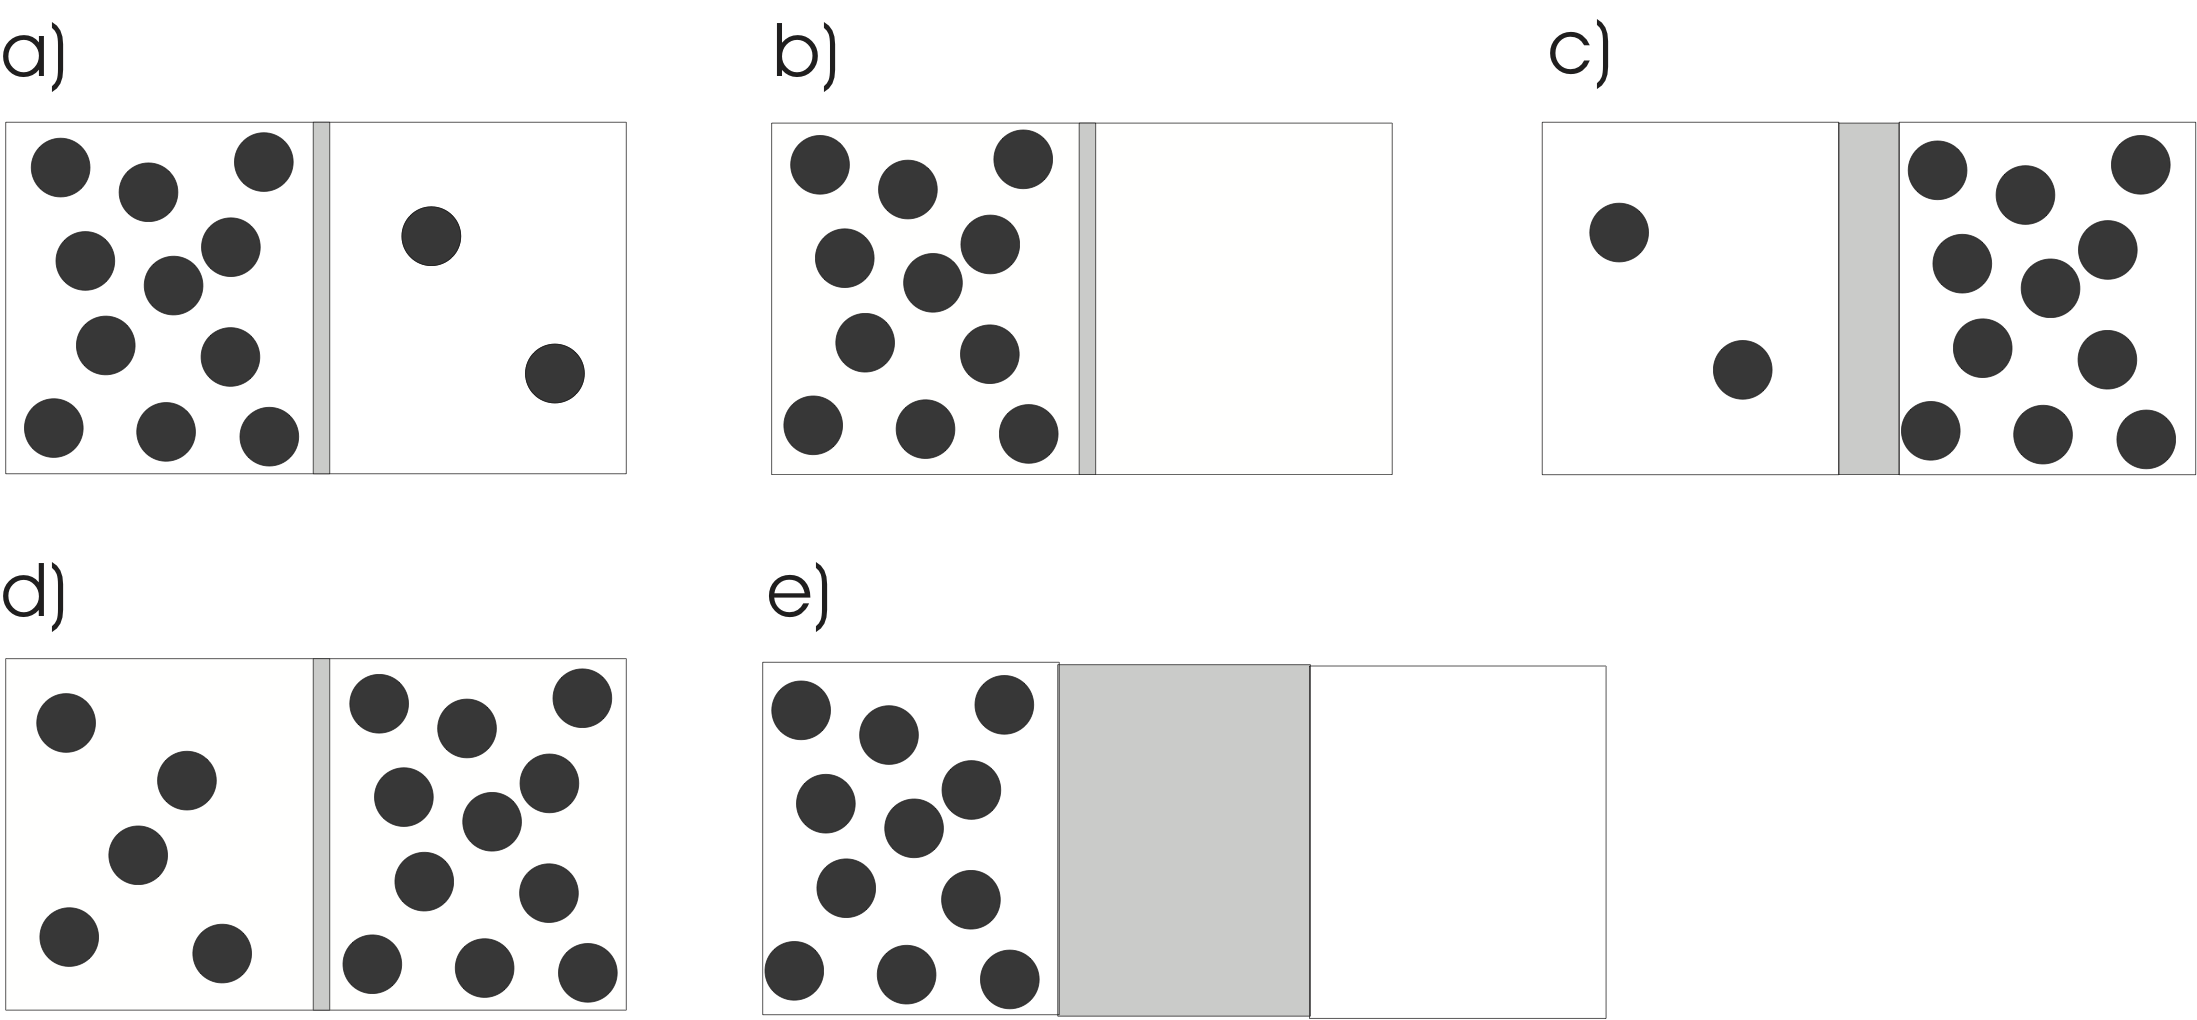
\includegraphics[width=0.5\textwidth]{../../../questions/E/images/Diffusion.png}

\begin{choices}
	\choice d)
	\choice e)
	\choice c)
	\choice b) (correct)
	\choice a)
\end{choices}

\vspace{3mm}\question Wie ändert sich der Diffusionsfluss \( J \) durch eine kreisförmige Membran, wenn deren Durchmesser sich verdoppelt?

\begin{choices}
	\choice \( J \) vervierfacht sich. (correct)
	\choice \( J \) ist unabhängig vom Durchmesser der Membran.
	\choice \( J \) quadriert sich.
	\choice \( J \) verdoppelt sich.
	\choice \( J \) halbiert sich.
\end{choices}

\vspace{3mm}\question Der Diffusionsfluss beschreibt ...

\begin{choices}
	\choice die transportierte Stoffmenge pro Fläche.
	\choice die transportierte Stoffmenge pro Volumen.
	\choice die transportierte Stoffmenge.
	\choice die transportierte Stoffmenge pro Zeit und Fläche.
	\choice die transportierte Stoffmenge pro Zeit. (correct)
\end{choices}

\vspace{3mm}\question Welche Einheit ist zur Angabe von Konzentrationen NICHT möglich?

\begin{choices}
	\choice \( \frac{kmol}{l} \)
	\choice \( mol \cdot cm^{-3} \)
	\choice \( kmol \cdot m^{-3} \)
	\choice \( \frac{mol}{m^3} \)
	\choice \( l \cdot mol^{-1} \) (correct)
\end{choices}

\vspace{3mm}\end{questions}

\end{document}
